\section{Experiments}
We run experiments on the dataset Study10 from the University of Virginia on electricity disaggregation. 
This dataset collects data from 02/10/2014 to 02/21/2014 in a residential building. 
%the following paragraph is from UVa
Two individuals were asked to live in an instrumented home for around two weeks. 
To ensure the data consisted of the personal usage patterns of the participants, 
they were encouraged to live in and use the home as they normally would use their own. 
%The study had institutional review board (IRB) approval and each participant received a \$100 incentive. 
An eMonitor \cite{eMonitor} sensor was used to collect both mains data for testing and circuit-level information for ground truth. 
Additional data, such as the opening of appliance doors and the flicking of light switches, 
was collected to provide sub-circuit level ground truth information for events such as lights.
Both the two-phase aggregated data and each device's data are collected at intervals of 2-3 seconds.
In total, 25 devices were connected to two phases at the entry of the house. 
Five of these devices are seldomly operated; less than five times. 
Fourteen devices consume power less than 100W, and the majority of them are lights. 
The largest power consumption of these devices is 11000W by indoor heating. 
The noise caused by the heating device is large; greater than 100W. 
Therefore we focus on disaggregating the six major electronic devices 
with power levels greater than 100W. 
 
% the datasets from University of Virginia on both water and electricity disaggregation. 
%There are totally six data sets. The statistic of these six data set is listed in Table \ref{table_datasets}. 
%The recording interval of these datasets is 2 or 3 seconds. 
%A sensor is instrumented on each device to trace its ground truth operations. 
%\begin{table}[!t]
\renewcommand{\arraystretch}{1.3}
\caption{Electricity Dataset}
\label{table_datasets}
\centering
\begin{tabular}{|c|c|c|c|}
\hline
Data sets & Start date & End date & Duration (day) \\
\hline
\hline
Study 10 & 02-10-2014 & 02-21-2014 & 12\\
\hline
Study 11 & 01-27-2014 & 02-07-2014 & 12\\
\hline
Study 12 & 01-09-2014 & 01-21-2014 & 12\\
\hline
Study 13 & 12-23-2013 & 01-03-2014 & 12\\
\hline
Study 14 & 12-09-2013 & 12-20-2013 & 12\\
\hline
Study 101 & 06-09-2014 & 06-28-2014 & 20\\
\hline
\end{tabular}
\end{table}

\subsection{Electricity Disaggregation}
We assume that we know the power levels of each device. 
If the power levels of each device are unknown, 
we can use the sum of two-phase aggregated data and the on/off events of the 
ground truth to extract them. 
%In order to extract the power level of each device, 
We set a window size $w=30s$ ahead and behind of the ground truth events to match 
the aggregated data.
If there is only one power change in the aggregated data during these 60 seconds, 
this power level change must come from an on/off event of an electrical device. 
Usually, it takes around 2-5 seconds for an electrical device to reach
a steady power level. 
The on and off events reflect different durations for a device to 
reach a steady state. 
Therefore, we measure the minimal duration of the on event and off event 
of each device. 
After we go over all the aggregated data and ground truth on/off events, 
we run a Gaussian mixture model to model the positive power changes and negative power changes
independently. The means and standard deviations correspond to  the on/off event of each device. 
The power levels, standard deviation, and on/off duration of each device of dataset study10 are listed in Table \ref{table_study10results}.
\begin{table*}[!t]
\renewcommand{\arraystretch}{1.3}
\caption{Power Levels, Standard Deviation of Power Levels, On/off Duration, Connected Phases and Disaggregation Results of Electricity Devices from Study10.}
\label{table_study10results}
\centering
%\small
\footnotesize
%\scriptsize
\setlength\tabcolsep{2pt}
\begin{tabular}{|c|c|c|c|c|c|c|c|c|c|c|}
\hline
\multirow{2}{*}{Device} & Power & Standard & On/off &  \multirow{2}{*}{Phase} & \multicolumn{3}{|c|}{Recursive Multivariate Motif Mining} & \multicolumn{3}{|c|}{AFAMAP}\\
\cline{6-11}
           &  Levels & Deviation & Duration &  &Precision&  Recall &  F-measure & Precision & Recall & F-measure\\ 
\hline
\hline
\multirow{2}{*}{HeatingIndoor+} & \multirow{2}{*}{10590W} & \multirow{2}{*}{1270W} & \multirow{2}{*}{60s} & \multirow{2}{*}{1+2} & \multirow{2}{*}{0.979} & \multirow{2}{*}{0.928} & \multirow{2}{*}{0.953} & \multirow{2}{*}{0.870}& \multirow{2}{*}{0.45} & \multirow{2}{*}{0.598}\\
HeatingOutdoor &  &  &  &  &  &  &  &  & & \\
\hline
Waterheater & 4450W & 350W &  2-5s & 1+2 & 0.999 & 0.997 &0.998 &0.627& 0.882 &0.733\\
\hline
Humidifier & 1470W & 90W & 10s & 1 & 0.997 & 0.992 &0.995 & 0.725 & 0.858 & 0.787\\
\hline
Microwave & 1850W & 200W & 10s & 2 & 0.95 &0.758 & 0.843 & 0.032 & 0.819 & 0.06\\
%\hline
%HeatingOutdoor & 4446W & 140 W & 2-18s & 1+2 &0.308 & 0.66& 0.42& & &\\
\hline
\multirow{2}{*}{Dryer} & 5200W &400W & 2-5s & 1+2 & \multirow{2}{*}{0.911}&\multirow{2}{*}{0.996}&\multirow{2}{*}{0.952}& \multirow{2}{*}{0.011}&\multirow{2}{*}{0.561} & \multirow{2}{*}{0.021}\\
\cline{2-3} \cline{4-5}
                       & 875W &225W  & 2-5s & 1 & & & & & &\\
%\hline
%L007 & 239W & 56W &  2-5s &2 & & & & & &\\
%\hline
%Fridge & 102W & 68W & 2-5s &1& - & - & - & & &\\
%\line
%L010 & 92W & 16W & 2-5s &2& & & & & &\\
%\cline
%L011 & 117W & 29W & 2-5s &1& & & & & &\\
%\hline
%L012 & 104W & 28W & 2-5s & 2& & & & & &\\
\hline
\end{tabular}
\end{table*}


%By analyzing each device, we notice that sometimes the power levels and 
%on/off duration are insufficient to identify the electric devices. 
%For instance, when the device heatingIndoor starts alone, 
%it takes $2-5$ seconds to go to a steady state as shown in Figure \ref{fig_heatingDevices} (a).
%But when the combined device of heatingIndoor and heatingOutdoor 
%starts, the starting duration takes around $4-18$ seconds. 
%In Figure \ref{fig_patterns} (b), after this combined device 
%starts for15 seconds, the power levels changes 
%for 9 times then to a relatively stable state. 
%During this period of 15 seconds, the power changes very rapidly. 
%If we accumulate these power levels together, 
%it's not a fix number. Therefore, for this kind of device, 
%we can only compare the shape of the startup to decide the on events 
%from the aggregated data. 

We apply recursive multivariate piecewise motif mining to dataset Study10 
and compute the precision, recall and F-measure. 
Devices which draw power from both phases are separated first. 
They are heatingIndoor, waterheater and dryer.
\begin{figure*}[!t]
        \centering{
                \begin{tabular}{cc}
                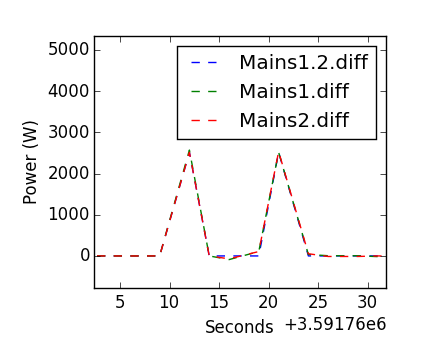
\includegraphics[width=3.2in]{multidisaggfig/heatingIndoorPhase12On.png} &
                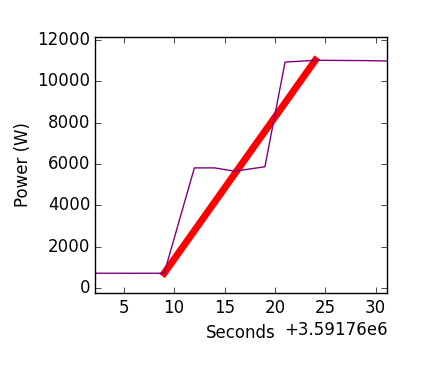
\includegraphics[width=3.2in]{multidisaggfig/heatingIndoorUp.png} &
                (a) & (b) \tabularnewline
                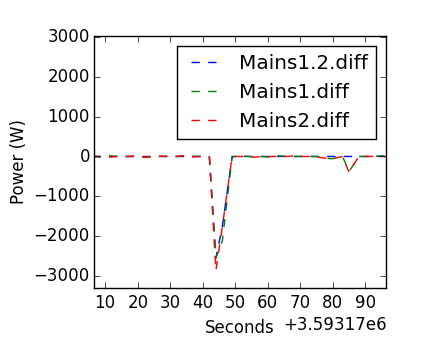
\includegraphics[width=3.2in]{multidisaggfig/heatingIndoorPhase12Off.png} &
                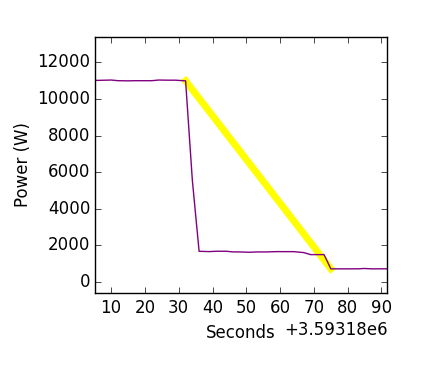
\includegraphics[width=3.2in]{multidisaggfig/heatingIndoorDown.png}\tabularnewline
                (c) & (d) \tabularnewline
                \end{tabular}
                }
        \caption{
        (a) On piecewise event and (c) Off piecewise event of heatingIndoor. heatingIndoor is disaggregated by motif mining the on event (b) and off event (d).}
        \label{fig_heatingIndoorResults}
\end{figure*}

Figure \ref{fig_heatingIndoorResults} (a) gives an example of 
an on event in the two-phase Mains1 and Mains2. 
Mains1.diff denotes the diffs data from Mains1 and Mains2.diff represents 
the diffs data from Mains2. 
Mains1.2.diff shows as blue when Mains1 and Mains2 share the similar power changes. 
We can see that 
the power consumption of a specific device jumps twice in two phases simultaneously.
The first time, both phases jump 2572W. After nine seconds, 
the power of both phases increases  2520W. 
The sum of these four changes is 10184W. 
Compared with the power levels of all devices, 
we speculate that these power changes are caused 
by the device heatingIndoor. 
%By applying multivariate piecewise motif mining, 
%we match the power consumption with $11000W$ and 
%categorize this on event into heating indoor. 
Figure \ref{fig_heatingIndoorResults} (b) shares the same snippet of time series as Figure \ref{fig_heatingIndoorResults} (a). 
The red line indicates that the on event of heatingIndoor is recognized.    
\begin{figure*}[!t]
        \centering{
                \begin{tabular}{cccc}
                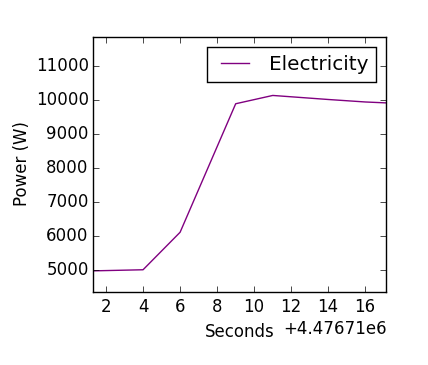
\includegraphics[width=3.2in]{multidisaggfig/dryerPhase_sum.png} &
                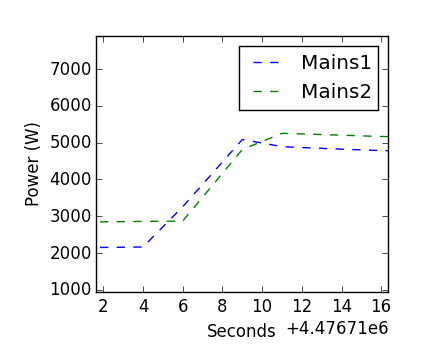
\includegraphics[width=3.2in]{multidisaggfig/dryerPhase12On.png} \tabularnewline
                (a) & (b) \tabularnewline
                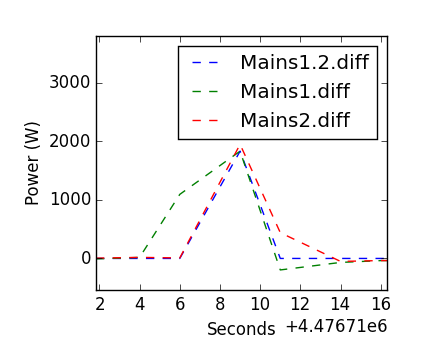
\includegraphics[width=3.2in]{multidisaggfig/dryerPhase12OnDiff.png} &
                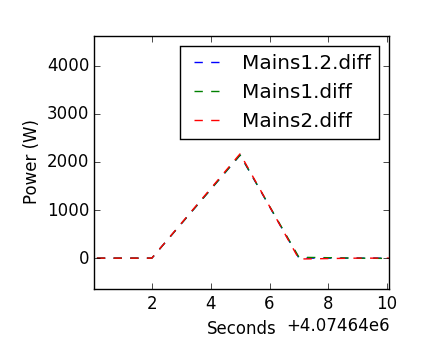
\includegraphics[width=3.2in]{multidisaggfig/waterHeaterPhase12OnDiff.png}\tabularnewline
                (c) &(d) \tabularnewline
                \end{tabular}
                }
        \caption{
        Disaggregating dryer with multivariate motif mining.
        (a) the startup in the sum of aggregated power (b) the startup in two phases (c) the diffs in two phases on event of dryer.
        (d) the diffs in two phases on event of water heater which shares same power level as dryer but different patterns when drawing power from two-phases.
        }
        \label{fig_dryerResults}
\end{figure*}

Similarly, the off event plunges twice in two seconds -2877W and -1759W in both phases, as shown in Figure \ref{fig_heatingIndoorResults} (c).
The sum of this off event is -9272W. 
After matching the power levels, we categorize it as the off event of heatingIndoor as indicated in Figure \ref{fig_heatingIndoorResults} (d). 

The dryer has the same power level as the waterheater at around 4800W. 
If we disaggregate these two devices from the sum of the two phases, 
it's difficult to distinguish them,  
but with multivariate piecewise motif mining, these two devices 
can be distinguished. 

%Figure \ref{fig_dryerResults} (a) and (b) shows the on event of dryer from sum of phase 1 and phase 2, 
%and these two phases separately. 
Figure \ref{fig_dryerResults} (a) and (b) are the diff data of the dryer and waterheater from the two-phase circuit. 
We can see that the waterheater draws power from Phase 1 and Phase 2 at the same time,  
but the dryer shows a different pattern. It draws power from Phase 1 at a lower power of 1093W, then jumps to 1830W; 
at the same time, it draws power from Phase 2 at the high level of 1946W immediately. 
We encode the power usage as shown in Figure \ref{fig_eventEncoding}, then apply motif mining to disaggregate them. 
 
After deleting the power consumption from both aggregated phases, 
we apply piecewise motif mining again to a single phase. 
We then discover the humidifier from Phase 1 
and the microwave from Phase 2. 
%Note that the power consumption of humidifier and microwave overlaps sometimes, 
%which makes it hard to separate them. 
%But they draw power from different phases separately. 
%Multivariate motif mining can separate them. 
When we only disaggregate the sum of Phase 1 and Phase 2, 
the precision recall result of the microwave and humidifier is not very accurate 
because sometimes their power consumptions are similar. 
However, using multivariate motif mining, we can separate them very clearly 
with good precision and recall. 
The precision and recall results for the data set Study10 are listed in Table \ref{table_study10results}.

Recursive multivariate motif mining is capable of disaggregating continuous variable loads. 
%\begin{figure*}[!t]
        \centering{
                \begin{tabular}{cccc}
                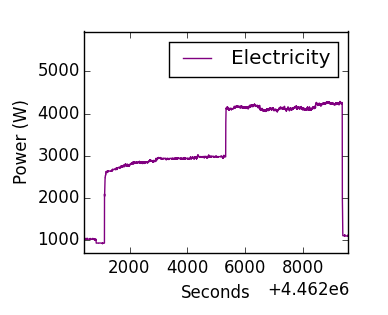
\includegraphics[width=3.2in]{multidisaggfig/heatingIndoorOutdoorPattern1_sum.png} &
                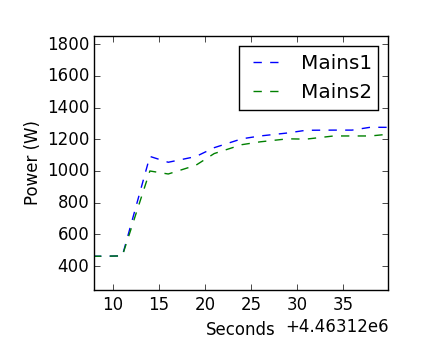
\includegraphics[width=3.2in]{multidisaggfig/heatingIndoorOutdoorPattern1.png} \tabularnewline
                 (a) & (b)\tabularnewline
                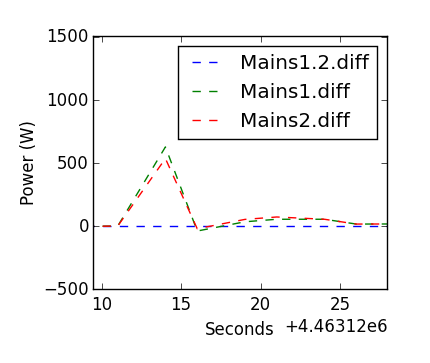
\includegraphics[width=3.2in]{multidisaggfig/heatingIndoorOutdoorPhase12On_1.png} &
                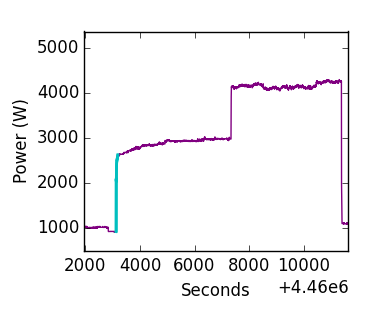
\includegraphics[width=3.2in]{multidisaggfig/heatingIndoorOutdoorFittedPattern1.png}\tabularnewline
                (c) &(d) \tabularnewline
                \end{tabular}
                }
        \caption{
        Disaggregating continuous variable load heating outdoor. 
        (a) the startup in the sum of aggregated power (b) the startup in two phases (c) the diffs in two phases (d) the disaggregated on event of heating outdoor.}
        \label{fig_heatingOutdoorResults}
\end{figure*}

Figure \ref{fig_dryerResults} (c) shows the diff data of heatingOutdoor from the two phases. 
During this on event, its power levels change nine times, then continue at a relatively stable state.
%Figure \ref{fig_heatingOutdoorResults} (a) illustrates the startup of heatingOutdoor.
%as shown in Figure \ref{fig_heatingOutdoorResults} (b) and (c). 
By applying piecewise motif mining, 
we can successfully identify this as the heatingOutdoor device 
after matching its power level. 
%The disaggregated result is displayed in Figure \ref{fig_dryerResults} (d).
%Note that this continuous variable load startup snippet can be discovered by dynamic time warping 
%subsequence search as well if this device is on without the intervene of other devices.
If another device  $D$ which draws from Phase 1 or Phase 2 is turned on or off during this period, 
multivariate piece-wise motif mining can still identify this heatingOutdoor device. 
This is because $D$ only uses one phase's power; 
hence its power change is not counted in our piecewise event. 
